\chapter{合成策略与绿色化学}\label{ch:g12:synthesis-strategy}

同一种止痛药布洛芬已有两种制法。较早的
路线需要六步，每采购一百千克起始原料，
就有六十千克最终变为废物。较新的路线需要三步，
几乎保留了所采购的每一个原子。两种方法得到的药片中白色粉末相同，
区别只在于规划。制定合成方案的化学家会提出四个问题：
如何快速完成，如何获得较多产物，如何只作用于分子的正确部位，
以及如何尽量少产生废物。

\begin{recall}
合成包括反应、分离、提纯和鉴定；其
产率（\cref{ch:g10:synthesis-yield}）。弯箭头、取代、
加成、消除（\cref{ch:g12:curly-arrows}）。催化剂能加快
反应，而自身不被消耗（\cref{ch:g12:catalysis}）。非完全反应在
$Q = K$ 时停止；加入过量的反应物，或移去生成物，
可使其继续进行（\cref{ch:g12:equilibrium}）。
\end{recall}

\begin{omfigure}
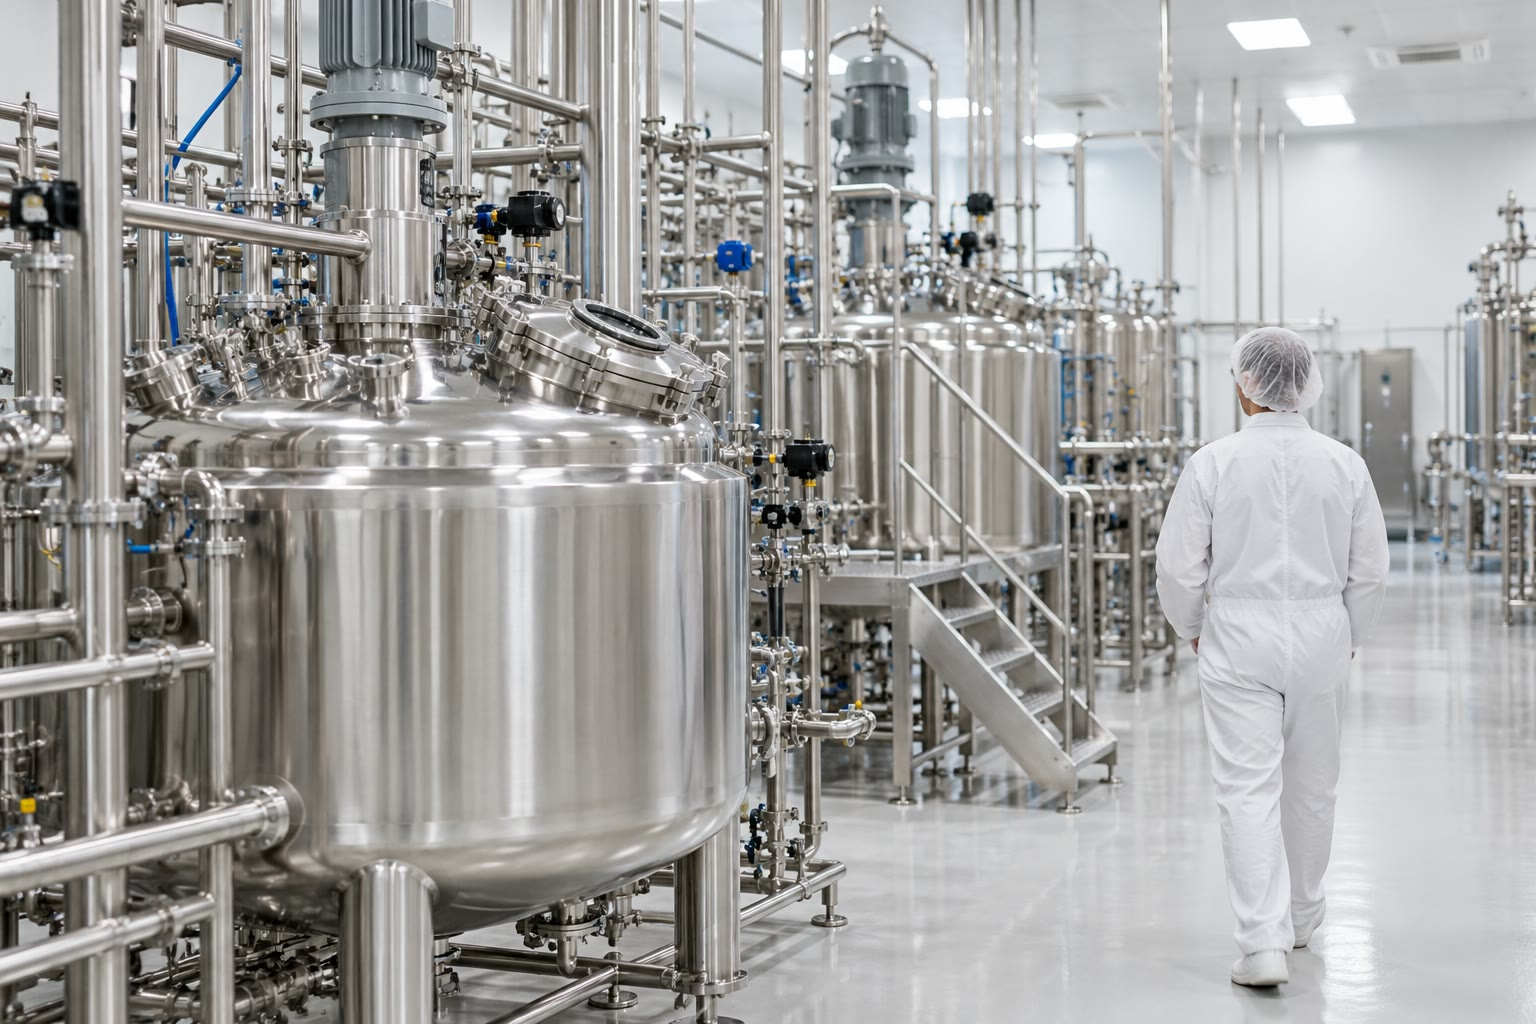
\includegraphics[width=0.48\linewidth]{images/book1/ai/g12-pharma-plant.jpg}

{\small 一座制药厂：合成所用的反应器，规模放大至
吨级。}
\end{omfigure}

\section{优化合成方案}

可改进两个不同的量：\emph{反应速率}，它决定合成
需要多长时间；另一个是\emph{产率}，它决定合成
得到多少产物。

\begin{proposition}[影响反应速率与产率的因素]\label{prop:g12:synthesis-strategy:levers}
\begin{itemize}
  \item 反应速率随温度升高、随反应物浓度增大，
        并随催化剂的加入而加快。
  \item 完全反应的产率由限量反应物决定；
        非完全反应的产率则随某一反应物过量
        或随生成物一边生成一边被移去而增大。
        催化剂不改变产率，它只是使体系更快地
        达到相同的最终状态。
\end{itemize}
\end{proposition}

\begin{proof}
第一条归纳了
\cref{ch:g12:reaction-rates,ch:g12:catalysis}中的动力学因素。
非完全反应结束时 $Q = K$，加入反应物或移去
生成物会使 $Q < K$，反应继续向正向进行。
\end{proof}

\begin{example}[带分水器的酯化反应]\label{ex:g12:synthesis-strategy:trap}
乙酸与乙醇各 1 摩尔，
平衡时仅得到 \qty{67}{\percent} 的酯。若将混合物
在不与水混溶的溶剂中加热回流，并加入少量
酸作催化剂，蒸气冷凝后进入侧管，形成
\emph{分水器}：水密度较大，沉在底部并留在那里，
溶剂则回流入烧瓶。水在生成时即离开反应体系，
因此 $Q$ 保持小于 $K$，酯化反应几乎进行到底。
加热提高反应速率，催化剂使速率更快，分水器则提高
产率。
\end{example}

\begin{omfigure}
\begin{tikzpicture}[font=\small, scale=0.8]
  \pic[transform shape] at (0,0) {hotplate};
  \pic[transform shape] at (0,0) {rbflask={0.55}{orange!20}};
  % the trap: water at the bottom, solvent above, up to the arm
  \fill[cyan!60!blue!40] (1.0,1.75) arc[start angle=180, end angle=360, radius=0.15] -- (1.3,2.3) -- (1.0,2.3) -- cycle;
  \fill[yellow!35] (1.0,2.3) rectangle (1.3,3.25);
  \draw[om glass] (-0.2,3.0) -- (-0.2,3.75) -- (0.2,3.75) -- (0.2,3.55) -- (1.0,3.55) -- (1.0,4.0);
  \draw[om glass] (0.2,3.0) -- (0.2,3.25) -- (1.0,3.25) -- (1.0,1.75) arc[start angle=180, end angle=360, radius=0.15] -- (1.3,4.0);
  \pic[transform shape] at (1.15,4.0) {condenser};
  \draw[omProp, thick, <-] (1.35,2.0) -- (2.6,1.7) node[right, text=black, align=left] {水在底部 \\聚集};
  \draw[omProp, thick, <-] (1.35,2.9) -- (2.6,3.1) node[right, text=black, align=left] {溶剂溢流回 \\烧瓶};
  \draw[omProp, thick, <-] (-0.6,0.6) -- (-1.7,1.1) node[left, text=black, align=right] {乙酸、乙醇、\\催化剂、溶剂};
\end{tikzpicture}

{\small 回流加热的烧瓶上装有分水器：生成的水
在冷凝时从反应体系中被移出。}
\end{omfigure}

\section{选择性}

实际分子中常含有若干官能团。若某试剂
能同时作用于它们全部，便会得到混合物；
好的合成则选用只作用于待改变官能团的试剂。

\begin{definition}[化学选择性反应]\label{def:g12:synthesis-strategy:chemoselective}
若一个反应的试剂作用于含多个官能团的分子时，
只改变其中一个官能团、保持其余部分不变，
则称该反应为\emph{化学选择性反应}\index{化学选择性反应}。
\end{definition}

\begin{example}[有选择性的还原剂]\label{ex:g12:synthesis-strategy:nabh4}
硼氢化钠 \ce{NaBH4} 可将醛和酮的羰基
还原为醇羟基，但不影响酯。在同时含有酮和
酯的分子上，只有酮发生改变：
\[
  \ce{CH3-CO-CH2-CH2-CO-O-CH3}
  \;\xrightarrow{\ \ce{NaBH4}\ }\;
  \ce{CH3-CH(OH)-CH2-CH2-CO-O-CH3} .
\]
较强的还原剂氢化铝锂 \ce{LiAlH4} 会同时还原
两个官能团，因此它在此处不具有化学选择性。
\end{example}

\begin{remark}[选择性的几种类型]\label{rem:g12:synthesis-strategy:kinds}
化学选择性是在不同官能团之间进行选择。反应还可以在同一
官能团的两个位置之间进行选择，或在生成物的两种立体异构体之间选择，
正如\cref{ch:g12:catalysis}中的酶，以及
\cref{ch:g12:stereochemistry}中的手性分子所示。
每一类都将在本科分册中学习。
\end{remark}

\section{保护基}

当没有试剂的选择性足够高时，化学家会先将不应参与反应的官能团遮蔽起来，
进行反应，然后再使该官能团复原。

\begin{definition}[保护基]\label{def:g12:synthesis-strategy:protecting-group}
称\emph{保护基}\index{保护基}为连接在
官能团上、以阻止其在合成的一步或多步中发生反应的基团，
并可在之后移除，以复原原来的官能团。三种操作分别是
\emph{保护}、\emph{反应}和
\emph{脱保护}。
\end{definition}

\begin{method}[设计保护方案]\label{met:g12:synthesis-strategy:plan}
\begin{enumerate}
  \item 列出每种反应物所含的官能团，以及需要形成的那一个化学键。
  \item 标出该步试剂也可能进攻的
        其他官能团。
  \item 用能耐受反应条件的保护基保护它们，
        且该保护基可在温和条件下除去，
        同时保持新形成的化学键完好。
  \item 计算代价：每次保护会增加两步，即保护与
        脱保护，并降低总产率。
\end{enumerate}
\end{method}

\begin{example}[制备一种二肽，而非四种]\label{ex:g12:synthesis-strategy:dipeptide}
甘氨酸 \ce{H2N-CH2-COOH} 和丙氨酸 \ce{H2N-CH(CH3)-COOH}，各自都含一个
氨基和一个羧基。甘氨酸的羧基与丙氨酸的氨基之间形成酰胺键，
得到二肽 Gly--Ala。若将两者直接混合，
两种氨基酸会生成四种二肽，即 Gly--Ala、Ala--Gly、
Gly--Gly 和 Ala--Ala，混合物难以分离。方案如下：
\begin{enumerate}
  \item 用写作 \ce{Z} 的基团保护甘氨酸的氨基，并将
        丙氨酸的羧基保护为甲酯；
  \item 形成酰胺键：此时只有一个羧基和一个氨基
        保持游离；
  \item 去除两个保护基。
\end{enumerate}
\end{example}

\begin{omfigure}
\begin{tikzpicture}[font=\small, node distance=0.55cm,
    box/.style={draw=omDef, rounded corners=2pt, fill=omDef!6, align=center, inner sep=4pt}]
  \node[box] (a) {\ce{H2N-CH2-COOH}\\ \ce{H2N-CH(CH3)-COOH}};
  \node[box, below=of a] (b) {\ce{Z-NH-CH2-COOH}\\ \ce{H2N-CH(CH3)-CO-O-CH3}};
  \node[box, below=of b] (c) {\ce{Z-NH-CH2-CO-NH-CH(CH3)-CO-O-CH3}};
  \node[box, below=of c] (d) {\ce{H2N-CH2-CO-NH-CH(CH3)-COOH}};
  \draw[->, thick, omProp] (a) -- node[right, xshift=3pt, text=black] {1. 保护} (b);
  \draw[->, thick, omProp] (b) -- node[right, xshift=3pt, text=black] {2. 反应：形成酰胺键} (c);
  \draw[->, thick, omProp] (c) -- node[right, xshift=3pt, text=black] {3. 脱保护} (d);
  \node[anchor=east, font=\footnotesize, text=black!70] at ([xshift=-6pt]a.west) {甘氨酸、丙氨酸};
  \node[anchor=east, font=\footnotesize, text=black!70] at ([xshift=-6pt]d.west) {甘–丙二肽};
\end{tikzpicture}

{\small 保护、反应、脱保护：唯一能够
形成的酰胺键正是所需要的那一个。}
\end{omfigure}

\section{原子经济性}

产率为 \qty{100}{\percent} 表示每一个限量反应物分子
都转化为了生成物，但它并不能说明所购入的原子中，
有多少进入了生成物。方程式中的其他生成物，
无论多么纯净，若无人加以利用，便是废物。

\begin{definition}[原子经济性]\label{def:g12:synthesis-strategy:atom-economy}
某一合成的\emph{原子经济性}\index{原子经济性}是指
按配平方程式的比例取用的反应物质量中，
最终进入目标生成物的那部分所占的比例。
\end{definition}

\begin{proposition}[由方程式求原子经济性]\label{prop:g12:synthesis-strategy:atom-economy}
对于配平方程式 $a_1\,\ce{R1} + a_2\,\ce{R2} + \cdots \rightarrow
p\,\ce{P} + \text{其他生成物}$，
\[
  \text{原子经济性} =
  \frac{p\,M(\ce{P})}{a_1 M(\ce{R1}) + a_2 M(\ce{R2}) + \cdots}
  \times 100\,\% .
\]
\end{proposition}

\begin{proof}
若反应进行了 $x$ 摩尔，则消耗的反应物质量为
$x\,(a_1 M(\ce{R1}) + \cdots)$，生成的目标生成物质量为
$x\,p\,M(\ce{P})$；二者之比与 $x$ 无关。
\end{proof}

\begin{method}[计算原子经济性]\label{met:g12:synthesis-strategy:atom-economy}
\begin{enumerate}
  \item 写出配平方程式；若路线包含多步，则将各步相加，
        使每个中间体都被消去。
  \item 计算各反应物和目标生成物的
        摩尔质量。
  \item 代入公式，并使用化学计量数。
  \item 每千克目标生成物产生的废物质量为
        $(100 - \text{原子经济性})/\text{原子经济性}$ 千克。
\end{enumerate}
\end{method}

\begin{example}[加成与取代的比较]\label{ex:g12:synthesis-strategy:compare}
% ledger: aw:C, aw:H, aw:Br, aw:Na, aw:O
由乙烯制得溴乙烷，\ce{C2H4 + HBr -> C2H5Br}：每个原子都
进入了生成物，原子经济性为 $108.9/(28.0 + 80.9) = \qty{100}{\percent}$。
由溴乙烷制得乙醇，\ce{C2H5Br + NaOH -> C2H5OH + NaBr}：
原子经济性为 $46.0/(108.9 + 40.0) = \qty{30.9}{\percent}$；每千克乙醇
会副产 \qty{2.2}{kg} 溴化钠。加成反应的
原子经济性总为 \qty{100}{\percent}；取代反应和消除反应
则永远达不到。
\end{example}

\begin{omfigure}
\begin{tikzpicture}
\begin{axis}[width=0.8\linewidth, height=5.2cm, ybar, bar width=16pt,
    ymin=0, ymax=112, ylabel={原子经济性（\%）},
    xtick={1,2,3,4,5}, xticklabels={加成，酯化，布洛芬（3 步），布洛芬（6 步），取代},
    xticklabel style={font=\footnotesize, align=center, text width=2.1cm},
    nodes near coords, nodes near coords style={font=\footnotesize},
    enlarge x limits=0.12, axis lines*=left, ymajorgrids, grid style={black!12}]
  \addplot[fill=omDef!55, draw=omDef] table[x=i, y=AE] {figdata/out/grade-12-synthesis-strategy.dat};
\end{axis}
\end{tikzpicture}

{\small 由方程式算得的原子经济性：乙烯与溴化氢、
乙酸与乙醇、布洛芬的两条路线，以及
溴乙烷与氢氧化钠。}
\end{omfigure}

\section{绿色化学}

\begin{definition}[绿色化学]\label{def:g12:synthesis-strategy:green-chemistry}
\emph{绿色化学}\index{绿色化学}是指设计
化学产品与化工过程，以减少或消除有害物质的使用和
生产，并统筹考虑从起始原料的选择
直至产品使用后的去向。
\end{definition}

十二条原则概括了这一思路，每条都是
对一个过程应当提出的问题。
% ledger: green:12
\begin{enumerate}
  \item 先防止产生废物，而非事后治理。
  \item 最大化原子经济性。
  \item 设计危害更小的合成路线。
  \item 设计更安全的化学品和产品。
  \item 使用更安全的溶剂和反应条件。
  \item 提高能量效率：尽量在接近常温
        常压下操作。
  \item 使用可再生原料。
  \item 避免使用化学衍生物，如保护基。
  \item 使用催化剂，而不用化学计量的试剂。
  \item 设计使用后可降解的产品。
  \item 实时分析，以防止污染。
  \item 尽量降低发生事故的可能性。
\end{enumerate}

\begin{remark}[原则而非定律]\label{rem:g12:synthesis-strategy:principles}
这些原则常常相互矛盾：保护基违背原则 8，
却可能节省整个合成过程；能节约能量的催化剂，
也可能含有稀缺金属。评判一个过程，须权衡这些原则，
并尽量用数字说明：原子经济性、产率、废物质量、
能耗等。
\end{remark}

\begin{history}[绿色化学，1998 年]
% ledger: green:book-1998, ibu:bhc-commercial
1998 年，化学家保罗·阿纳斯塔斯和约翰·华纳出版了一本书，
\emph{绿色化学：理论与实践}一书，阐明了十二条
原则。就在前一年，一项政府颁发的绿色合成奖项
授予了布洛芬的三步合成路线，该路线自 1992 年起
已投入工业规模生产。此后，这些原则
便成为化学家职业训练的一部分。
\end{history}

\begin{example}[布洛芬的两条合成路线]\label{ex:g12:synthesis-strategy:ibuprofen}
% ledger: ibu:boots-steps, ibu:bhc-steps, ibu:boots-ae, ibu:bhc-ae, ibu:bhc-ae-recovered
布洛芬 \ce{C13H18O2} 由烃
\ce{C10H14}（异丁苯）制得。较老的路线共六步，
每一步都要用足量的试剂；合计起来，其反应物的
摩尔质量之和为 \qty{514.5}{g/mol}，得到 \qty{206.0}{g/mol} 的
布洛芬，原子经济性为 \qty{40}{\percent}。较新的路线共三步，
其中两步使用催化剂，总反应方程式为
\[
  \ce{C10H14 + C4H6O3 + H2 + CO -> C13H18O2 + C2H4O2}
\]
由此得 $206.0/266.0 = \qty{77}{\percent}$。其副产物乙酸，
经回收利用；若计为生成物，则原子经济性超过
\qty{99}{\percent}。
\end{example}

\begin{omfigure}
\chemfig{[:30]*6(-=(-[:90](-[:150])-[:30](=[:90]O)-[:-30]OH)-=-(-[:-90]-[:-150](-[:150])-[:-90])=)}

\medskip
\begin{tikzpicture}[font=\scriptsize,
    st/.style={draw=omDef, rounded corners=2pt, fill=omDef!6, minimum height=0.8cm, text width=1.15cm, align=center, inner sep=2pt}]
  \foreach \i/\t in {1/酰基化, 2/增加 2 个碳, 3/醛, 4/肟, 5/腈, 6/酸}
    \node[st] (o\i) at (1.7*\i,0) {\t};
  \foreach \i/\j in {1/2,2/3,3/4,4/5,5/6} \draw[->, thick] (o\i) -- (o\j);
  \node[anchor=east, align=right, font=\footnotesize] at ([xshift=-4pt]o1.west) {6 步 \\ \textbf{40 \%}};
  \foreach \i/\t in {1/酰基化, 2/加 \ce{H2}, 3/加 \ce{CO}}
    \node[st, fill=omProp!8, draw=omProp] (n\i) at (1.7*\i,-1.4) {\t\\ （催化剂）};
  \foreach \i/\j in {1/2,2/3} \draw[->, thick] (n\i) -- (n\j);
  \node[anchor=east, align=right, font=\footnotesize] at ([xshift=-4pt]n1.west) {3 步 \\ \textbf{77 \%}};
  \node[anchor=west, align=left, font=\footnotesize] at ([xshift=6pt]n3.east) {副产物：乙酸，已回收；\\ 计为生成物：超过 99 \%};
\end{tikzpicture}

{\small 布洛芬（上）及其两条工业合成路线：较老的一条
共六步；较新的一条共三步，均经催化，并附上各自的
原子经济性。}
\end{omfigure}

\begin{example}[更绿色的溶剂]\label{ex:g12:synthesis-strategy:solvents}
% ledger: crit:CO2-T, crit:CO2-p
许多反应与萃取过程都使用有毒、易燃或
易挥发的有机溶剂。当反应物能溶于其中时，水是最安全的
溶剂。二氧化碳也可以作为一种溶剂：高于
\qty{31}{\celsius}和\qty{73.8}{bar}时，它是一种\emph{超临界
流体}，既非液体也非气体，能溶解许多有机分子。
例如，它能从咖啡豆中萃取咖啡因；当压强
释放后，它便直接恢复为气体，不会在
产品中留下残留。
\end{example}

\begin{omfigure}
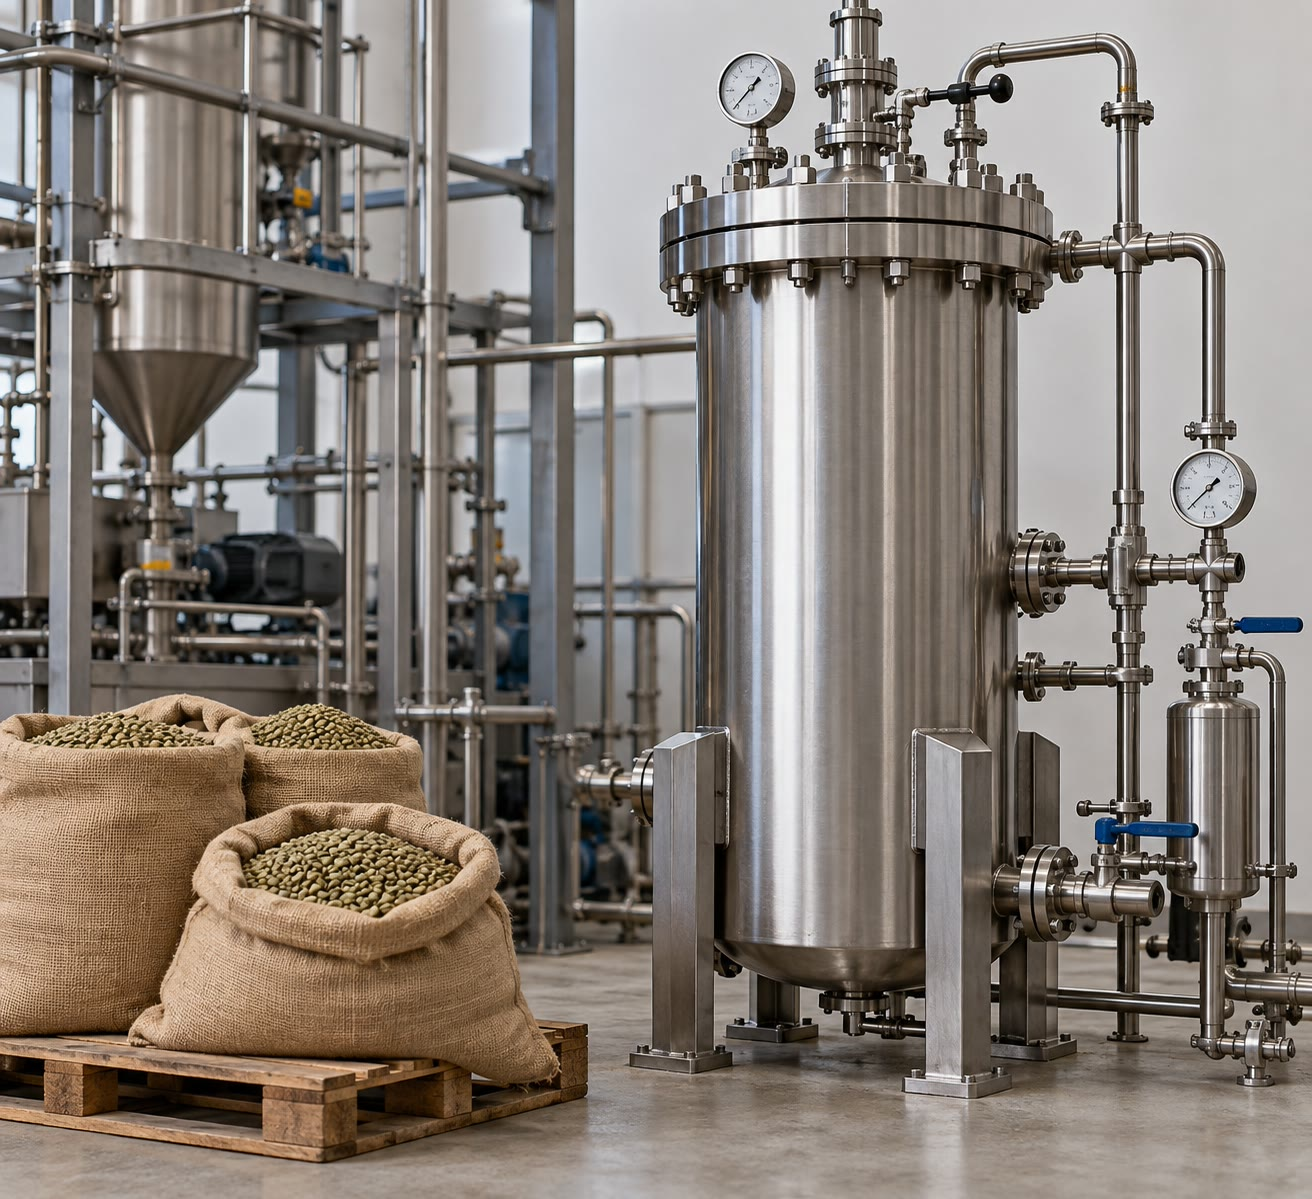
\includegraphics[width=0.45\linewidth,height=6cm,keepaspectratio]{images/book1/ai/g12-scco2-vessel.jpg}

{\small 高压萃取容器，其中超临界
二氧化碳取代了有机溶剂。}
\end{omfigure}

\section{练习}

\begin{exercise}[$\star$]\label{exo:g12:synthesis-strategy:1}
乙醇可由乙烯水合制得，\ce{C2H4 + H2O -> C2H5OH}，
或由葡萄糖发酵制得，\ce{C6H12O6 -> 2C2H5OH + 2CO2}。计算
二者各自的原子经济性。
\end{exercise}

\begin{exercise}[$\star$]\label{exo:g12:synthesis-strategy:2}
在本章的二肽合成方案中，指出每个保护基
被引入的步骤，以及被除去的步骤。
\end{exercise}

\begin{exercise}[$\star$]\label{exo:g12:synthesis-strategy:3}
某工厂在其一个反应中用水取代了氯代
溶剂。它应用了绿色化学的哪一条原则？
\end{exercise}

\begin{exercise}[$\star$]\label{exo:g12:synthesis-strategy:4}
为什么过量的乙醇能提高酯化反应的产率，
而催化剂却不能？
\end{exercise}

\begin{exercise}[$\star$]\label{exo:g12:synthesis-strategy:5}
硼氢化钠可还原醛和酮，但不还原酯。它与
4-氧代戊酸甲酯（同时含有酮与酯）的反应是否具有化学选择性？
哪一个官能团发生了变化？
\end{exercise}

\begin{exercise}[$\star\star$]\label{exo:g12:synthesis-strategy:6}
1 摩尔乙酸与 1 摩尔乙醇在平衡时生成 \qty{0.67}{mol}
的酯。提出两种提高该酯生成量的方法，以及一种
使反应更快达到平衡的方法。
\end{exercise}

\begin{exercise}[$\star\star$]\label{exo:g12:synthesis-strategy:7}
4-氧代戊酸甲酯，\ce{CH3-CO-CH2-CH2-CO-O-CH3}，先
用硼氢化钠处理一次，再用过量的
氢化铝锂处理一次，后者可将酯还原为两种醇。写出每种产物。
\end{exercise}

\begin{exercise}[$\star\star$]\label{exo:g12:synthesis-strategy:8}
在原子经济性的柱状图上，哪些反应保留了超过
四分之三的原子？布洛芬的三步路线相对于六步路线
优越多少倍？
\end{exercise}

\begin{exercise}[$\star\star$]\label{exo:g12:synthesis-strategy:9}
阿司匹林可由 \ce{C7H6O3 + C4H6O3 -> C9H8O4 + C2H4O2} 制得。计算其
原子经济性，以及每千克阿司匹林所产生副产物的质量。
\end{exercise}

\begin{exercise}[$\star\star$]\label{exo:g12:synthesis-strategy:10}
为什么合成反应要加热回流，而不是在敞口烧瓶中进行？
二者之中，加热提高的是反应速率还是产率？
\end{exercise}

\begin{exercise}[$\star\star$]\label{exo:g12:synthesis-strategy:11}
在两条布洛芬合成路线的示意图上，数一数各自的步骤数，
并说明较新的路线应用了绿色化学的哪些原则，至少给出三条。
\end{exercise}

\begin{exercise}[$\star\star\star$]\label{exo:g12:synthesis-strategy:12}
某三步合成的产率分别为 \qty{80}{\percent}，
\qty{70}{\percent} 和 \qty{90}{\percent}。计算总产率。
若要得到 \qty{0.10}{mol}
的最终产物，需要多少摩尔的起始原料？每 1 摩尔起始原料
至多生成 1 摩尔产物。
\end{exercise}

\begin{exercise}[$\star\star\star$]\label{exo:g12:synthesis-strategy:13}
规划二肽 Ala--Gly（由丙氨酸的羧基与甘氨酸的
氨基结合而成）的合成：需要保护哪些基团，
该方案需要几步？
\end{exercise}

\begin{exercise}[$\star\star\star$]\label{exo:g12:synthesis-strategy:14}
某公司称其工艺为“绿色”工艺，因为它使用了催化剂。该工艺
在 \qty{250}{\celsius} 下于苯中进行，苯是一种有毒溶剂，其原子经济性为
\qty{35}{\percent}。请
逐条依据绿色化学原则，判断该说法是否成立。
\end{exercise}

\begin{exercise}[$\star\star\star$]\label{exo:g12:synthesis-strategy:15}
咖啡豆中的咖啡因可用二氯甲烷萃取，二氯甲烷是一种
易挥发的氯代溶剂；也可用超临界二氧化碳萃取，条件约为
\qty{40}{\celsius} 与 \qty{100}{bar}。请解释后者为何处于
超临界状态，为何需要耐压性好的容器，并
给出它相对于前者的两个优点。
\end{exercise}

\section{问题：两条布洛芬合成路线}

\begin{problem}[{周末问题——三步路线每吨布洛芬
可避免多少废物？}]
\label{pb:g12:synthesis-strategy:1}
% ledger: ibu:boots-ae, ibu:bhc-ae, ibu:boots-steps, ibu:bhc-steps, aw:C, aw:H, aw:O, aw:N, aw:Cl, aw:Na
较早的布洛芬合成路线 \ce{C13H18O2} 需要六步。其反应物合计为
\ce{C10H14}、\ce{C4H6O3}、
\ce{C4H7ClO2}、\ce{C2H5ONa}、一种以 \ce{H3O} 计的酸、
\ce{NH3O} 以及两个 \ce{H2O}。较新的路线只需三步：
\[
  \ce{C10H14 + C4H6O3 + H2 + CO -> C13H18O2 + C2H4O2} .
\]

\medskip
\noindent\textbf{第一部分——方程式。}
\begin{enumerate}
  \item 检查较新路线的方程式在碳、
        氢、氧三种元素上是否配平。
  \item 指出较新路线的副产物名称。
  \item 在较早的路线中，反应物的哪些元素
        全部进入了废物？
  \item 两条路线中哪一条使用了催化剂？
        这应用的是哪一条原理？
\end{enumerate}

\medskip
\noindent\textbf{第二部分——原子经济性。}
\begin{enumerate}[resume]
  \item 计算布洛芬的摩尔质量。
  \item 计算较早路线
        反应物的摩尔质量之和。
  \item 推导其原子经济性。
  \item 计算较新路线
        反应物的摩尔质量之和。
  \item 推导其原子经济性。
  \item 若将乙酸计为生成物，
        则结果变为多少？
\end{enumerate}

\medskip
\noindent\textbf{第三部分——每吨废物。}
\begin{enumerate}[resume]
  \item 对于较早的路线，在 \qty{100}{\percent} 产率下，每吨布洛芬需购买
        多少质量的反应物？
  \item 每吨会产生多少质量的废物？
  \item 对较新路线提同样的问题：每吨反应物的质量。
  \item 每吨乙酸的质量。
  \item 若将乙酸计为废物，每吨可避免
        多少质量的废物？
\end{enumerate}

\medskip
\noindent\textbf{第四部分——产率与现实。}
\begin{enumerate}[resume]
  \item 假设每一步的产率均为 \qty{90}{\percent}，
        计算较早路线的总产率。
  \item 对较新路线做同样的计算。
  \item 除方程式外，再给出一个理由，说明
        步骤越少为何废物越少。
  \item 实际中乙酸会被回收利用。此时
        较新路线每吨产生多少质量的废物，
        \qty{100}{\percent} 产率下？
  \item 给出最终答案：三步路线每吨
        布洛芬可避免多少废物？
\end{enumerate}
\end{problem}
